\documentclass[12pt]{article}

\usepackage[a4paper, margin=1in]{geometry}
\usepackage{graphicx}

\setlength\parindent{0pt}
\setlength\parskip{1em}

\title{System Architectures \\ \bigskip Centralized Chat System}
\author{\textsc{Nguyen} Duc Tung \\ ICT.M7.003}
\date{\textsc{Tran} Giang Son - \textsc{Daniel} Hagimont \\ \medskip
March 26, 2018}

\begin{document}

\maketitle

\section{Introduction}

In this project, I developed a functional IRC system, with the required architecture. I tried to prevent and handle as many runtime errors could happen as I can. The system supports broadcast in a channel, send private message (PM) to a specific client. It also provides commands for client and server to utilise the system.

Both server and client work with multiplexed, nonblocking TCP socket connection.

\section{Client}

The client firstly takes server hostname from STDIN or from arguments, and then try to connect. After successfully connected, the program creates two separated threads: input handling thread, and network handling thread. Input thread send messages from keyboard to network thread through a pipe.

The pseudo design is as follows:

\begin{figure}
\centering
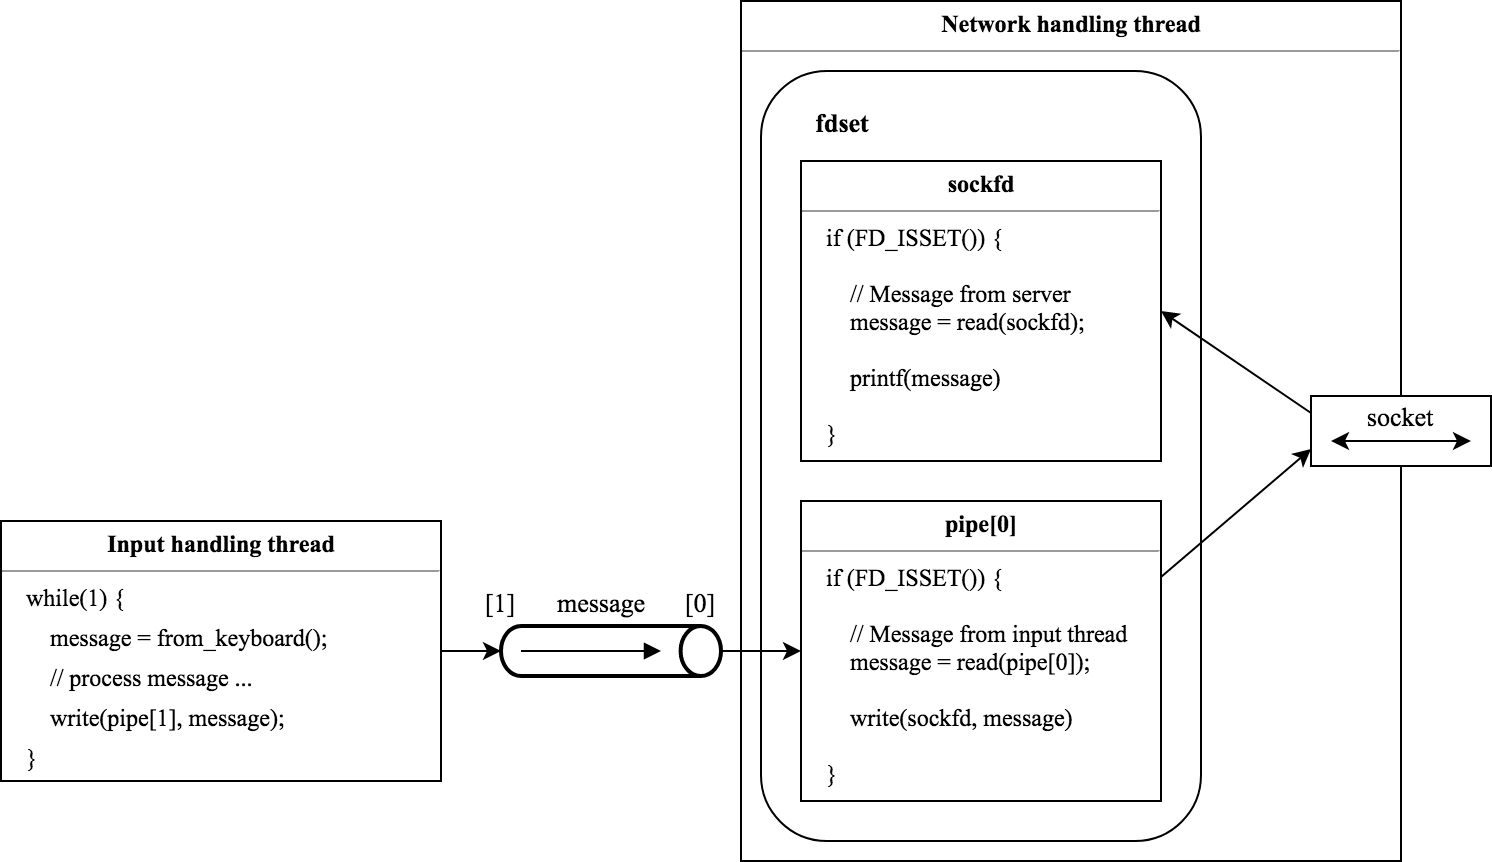
\includegraphics[width=\textwidth]{client_diagram.png}
\caption{Client's thread diagram}
\end{figure}

\subsection{Input handling thread}

\end{document}